%To submit to PCI for evaluation, you have to prepare a pdf file of all the contents pages of your paper, including the cover page: this behavior is triggered by removing the class option 'mode=plain' below.
%
%To transfer your PCI-recommended article to PCJ for publication, you have to prepare a pdf file without the cover page and header/footers: this behavior is triggered by the class option 'mode=plain' below. The cover page, including the metadata, the abstract, and the page headers/footers will be added upon online publication by the admin staff of the journal.
%
% This "author package" does not contain all the files necessary to support typesetting of a PCJ cover page. The cover page, including the metadata, the abstract, and the page headers/footers will be added upon online publication by the admin staff of the journal.

% add 'mode=plain' to transfer to PCJ
% remove 'mode=plain' to submit to PCI
\DocumentMetadata{tagging=on}
\documentclass[PCJ,Unicode,screen]{cedram}

\usepackage[
natbib=true,
mincitenames=1,
maxcitenames=2,
maxbibnames=20,
minbibnames=20,
uniquelist=false,
uniquename=false,
style=pcj
]{biblatex}
\usepackage{lipsum}
\usepackage{setspace}

% This is to correct wrong references sorting, see sample .bib file.
\providecommand*{\noopsort}[1]{}

% To suppress unwanted field in the bibliography:
\AtEveryBibitem{%
  \iffieldundef{doi}{}{%
  \clearfield{url}%
  \clearfield{urldate}%
  }%
  \clearfield{note}%
  \clearfield{publisher}%
  \clearfield{isbn}%
  \clearfield{issn}%
}

%%%%%%%%%%%%%%%%%%%%%%%%%%%%%%%%%%%%%%%%%%%%%%%%%%%%%%%%%%%%%
% Declare your BibTeX file here (keep the .bib extension):
\addbibresource{PCJ-sample.bib}

% Article metadata: these are useless when transferring your article to PCJ because they only appear on the cover page and article headers/footers after publication, and you are not asked/expected to generate these elements (there is a separate web interface to fill them in during the submission process).

\DOI{10.5802/fake.doi} % this is the DOI of the preprint on the preprint server
\PCIcorresp{charles.plessy@oist.jp}

\title[Pairwise genome alignment pipeline]{The nf-core/pairgenomealign pipeline for whole-genome alignments across the whole Tree of Life}

% Authors: me, the inerns, Nick, ask Martin, ask nf-core community, ask Nico, Jiashun?

%
 \author{\firstname{Charles} \lastname{Plessy}\IsEqualContrib}
 \address{Okinawa Institute of Science and Technology 1919-1 Tancha, Onna-son, Kunigami-gun Okinawa, Japan 904-0495}
 \email[Charles Plessy]{charles.plessy@oist.jp}
%
 \author{\firstname{Interns} \middlename{and} \lastname{Students}\IsEqualContrib}
 \address{Okinawa Institute of Science and Technology 1919-1 Tancha, Onna-son, Kunigami-gun Okinawa, Japan 904-0495}
 \email[TBD]{TBD@example.com}
%
 \author{\firstname{Nicholas} \middlename{M.} \lastname{Luscombe}}
 \address{Okinawa Institute of Science and Technology 1919-1 Tancha, Onna-son, Kunigami-gun Okinawa, Japan 904-0495}
 \email[Nichoasl M. Luscombe]{nicholas.luscombe@oist.jp}

 \keywords{pipline, Nextflow, nf-core, genome, alignment, synteny, ANI}
%
 \begin{abstract}

 - Only needs Nextflow and conda/docker/singularity

 - Aligns everything

 - Makes a pseudo MSA of all primate genomes in X hours.

 \end{abstract}
%
%%%%%%%%%%%%%%%%%%%%%%%%%%%%%%%%%%%%%%%%%%%%%%%%%%%%%%%%%%%%%%%%%%%%%%%%%%

\begin{document}

\maketitle
%you may choose to use a table of content
%\tableofcontents
\onehalfspacing

\section*{Introduction}

Recent advances in sequencing technologies, laboratory automation, and genome assembly algorithms have opened the prospect that chromosome-level genome assemblies may eventually become available for most known species. As genome assemblies become increasingly abundant, their comparison is emerging as a routine task for assembly quality control, variant discovery, evolutionary analysis, and large-scale comparative genomics. Although a rich ecosystem of specialised software exists for individual scientific questions, there remains a need for a generic workflow that prioritises ease of deployment, accessibility to non-specialists, reproducibility, robustness, and high-throughput execution. To address this need, we developed the \texttt{nf-core/pairgenomealign} pipeline using the Nextflow workflow system (\cite{Di_Tommaso_2017}) and the community standards, reusable modules, and software-distribution ecosystem provided by nf-core (\cite{Ewels_2020}; \cite{Langer_2025}).

We used the LAST software suite (\cite{Frith_2010}) for pairwise genome alignment because it accommodates a wide range of sequence lengths, divergences and compositional biases, while implementing an efficient seed-and-extend strategy with successive gapless and gapped extension until similarity fades. The key advantages of LAST are 1) its flexible seeding framework, which allows users to tune sensitivity and specificity through the design of exact or inexact seeds, including spaced, transition-constrained, and sparsely sampled seeds (\cite{Frith_2014}, \cite{Frith_2020}, \cite{Frith_2023}), 2) its training procedure that automatically infers substitution scores and gap penalties from the data, enabling robust alignment across queries with heterogeneous evolutionary distances (\cite{Hamada_2017}), and 3) its last-split program, which selects an optimal set of non-overlapping alignments to produce a consistent one-to-one mapping between genomes, thereby resolving multi-mapping regions in a principled manner (\cite{Frith_2015}), which avoids the need for post hoc chaining and netting strategies (\cite{Kent_2003}).

Several alternative pairwise alignment tools were considered, including LASTZ (\cite{Harris_2007}), MUMmer4 (\cite{Marcais_2018}), Minimap2 (\cite{Li_2018}), and, more recently, FastGA (\cite{Myers_2025}). LASTZ and MUMmer4 are widely used for whole-genome comparison, but neither combines the flexible seeding strategies, adaptive parameter training, and probabilistic split-alignment framework provided by LAST in a single integrated workflow. Minimap2 achieves excellent performance for read mapping and alignment of closely related long sequences but was not primarily designed for sensitive alignment of more diverged genomes. FastGA offers substantially improved speed for genome alignment; however, it became available after the core design and implementation of the present pipeline. We therefore selected LAST because it combined broad applicability across evolutionary distances with configurable sensitivity, data-driven parameter training, and principled resolution of ambiguous alignments.

Once computed, whole-genome alignments can be stored in formats that differ substantially in information content and storage efficiency. The Multiple Alignment Format (MAF), originally developed for the UCSC Genome Browser and related tools such as MULTIZ (\cite{Kent_2002a}; \cite{Blanchette_2004}), is the primary output format of LAST. In addition to alignment coordinates, MAF stores the aligned sequences and, in LAST, per-base alignment confidence values. More compact formats trade information for storage efficiency. The tabular output of LAST and the PSL format used by BLAT (\cite{Kent_2002b}) omit the alignment strings while retaining gap structure and summary statistics such as mismatch counts and gap openings. BLAST tabular output (\cite{Altschul_1990}) is more compact still, discarding the gap coordinates. At the end of the spectrum, alignments can be represented simply as paired genomic intervals in GFF or BED format with only an alignment score, providing near-maximal lossy compression in a text representation. Conversely, MAF alignments can be exported with minimal information loss to SAM/BAM (\cite{Li_2009}) and subsequently to CRAM format (\cite{Bonfield_2022}), benefiting from reference-based compression. The LAST suite can directly generate or export all of these formats.

TO Polish: we developped a draft of the pipeline in \cite{Plessy_2024}. It is now released as a nf-core pipeline. Here we report in details how it works and the improvements added in the meantime.

\section*{Methods }

\subsection*{Software deployment and versions}

The nf-core modules used in this pipeline rely on Free Software distributed through Bioconda (\cite{Gruening_2018}). Depending on the execution environment, these packages are installed automatically by Nextflow in isolated conda environments or provided through software containers. The default container sources are BioContainers (\cite{Leprevost_2017}; \cite{Bai_2021}), which maintain a one-to-one correspondence with Bioconda packages, and Wave containers (\cite{seqera_wave}), which can combine packages from both Bioconda and conda-forge (\cite{conda_forge_zenodo}) within a single image. Containers are distributed in Docker-compatible formats (\cite{DiTommaso_2015}) and can also be used through Singularity/Apptainer (\cite{Kurtzer_2017}), with BioContainers images converted and distributed by the Galaxy project (\cite{Afgan_2016}) and Wave images provided through Seqera. Container images may be cached locally and shared between users, reducing software installation overhead and improving reproducibility.

The nf-core modules implementing the LAST alignment workflow use several minimal containers with partially overlapping software dependencies. To avoid repeated downloads of redundant images, the \texttt{nf-core/pairgenomealign} pipeline overrides the default module configuration and provides a single shared container containing LAST v1651, samtools, htslib (\cite{Bonfield_2021}), and bcftools (\cite{Danecek_2021}) v1.23.1, open-fonts v0.7.0 from conda-forge (required for rendering sequence names in dotplots), gzip v1.14, bgzip v1.0.8, and xz v5.8.3.

\subsection*{Software configuration}

Software components are modularised through script templates that combine hard-coded tool arguments with configurable process parameters defined by the module maintainer. Configurable parameters are either linked directly to pipeline command-line options or passed through standard nf-core module variables, allowing users to modify or extend the resulting tool arguments via Nextflow configuration files. Resource settings that apply across modules, such as the number of CPU threads, are controlled through dedicated parameters.

Maximum execution times and memory allocations are assigned according to broad resource classes, ranging from lightweight to computationally intensive processes. These default settings can be overridden through standard Nextflow configuration mechanisms to match the requirements of specific computing environments.

\subsection*{Input}

Input genomes are provided in FASTA format and may optionally be compressed with gzip. When downstream outputs are generated in BAM, BCF, or CRAM format, the pipeline ensures that the corresponding reference genomes are available in the block-gzip (BGZF) format by recompressing them when necessary (\cite{Li_2011}). Existing BGZF-compressed files are reused unchanged. The use of BGZF enables the random-access indexing required by these output formats. The target genome, which will be indexed, is specified with the pipeline parameter \verb|--target|. We use \emph{target} rather than \emph{reference} because \emph{reference genome} commonly refers to a species' canonical genome assembly. Query genomes are specified through a sample sheet supplied via \verb|--input|. This table defines the collection of query genomes to be aligned against the target. As a convenience, a single query genome may alternatively be provided directly through the \verb|--query| parameter.

\subsection*{Alignment parameters}

Prior to database construction, any existing lowercase soft masking in the target genome is discarded and replaced with tandem-repeat masking using the tantan implementation embedded in LAST (\cite{Frith_2011}), using, \verb|lastdb|'s option \verb|--R01|. The maximal repeat unit length is hardcoded to 400~nt instead of \verb|lastdb|'s default of 100, to accommodate mammalian centromeric regions. Mask replacement can be disabled with the pipeline parameter \verb|--target|--softmask original|, which preserves the masking present in the input assembly.

The target database is indexed on both strands using the \texttt{lastdb} option \verb|--S2|. This increases memory usage during indexing but accelerates subsequent alignments. An important consequence is that some alignments may be reported between the reverse-complement strand of the target and the forward strand of the query, a representation that is not handled consistently by all downstream software. Users may therefore revert to single-strand indexing with the pipeline parameter \verb|--strand both|. The default seed scheme is \verb|RY4|, although alternative seeds can be selected through the \verb|--seed| parameter.

Alignment parameter training is performed with symmetric substitution scores and gap penalties by passing the \verb|--revsym|, \verb|--gapsym|, and \verb|--matsym| arguments to \texttt{last-train}. These constraints are appropriate for most nuclear genomes but may be undesirable when evolutionary processes differ between strands, such as in animal mitochondrial genomes. In such cases, advanced users can override the training arguments by redefining \texttt{ext.args} for the \texttt{ALIGNMENT\_TRAIN} process in a Nextflow configuration file. Alternatively, a predefined LAST parameter file may be supplied through the pipeline parameter \verb|--lastal_params|. The same parameter set is then applied to all query genomes. Such files may originate from a previous training run or correspond to a standard LAST scoring scheme.

By default, sequence alignments are computed with the \texttt{lastal} arguments \verb|-C2 -D1e9|, configurable through the pipeline parameter \verb|--lastal_args|. The \verb|-D1e9| setting specifies an effective genome size of 1~Gb for E-value calculations, whereas \texttt{-C2} prunes nested alignments in order to reduce the computational burden associated with highly repetitive regions such as centromeres. During the reduction of many-to-many alignments to one-to-one relationships, alignments with an estimated error probability greater than $10^{-5}$ are discarded. This threshold is controlled by the pipeline parameter \verb|--last_split_mismap|.

Multi-threaded LAST processes are allocated up to 12 CPU cores, subject to any lower limit imposed by user settings or institutional execution profiles. Thread count is not expected to affect alignment results, but it may alter the order in which alignments are reported. Consequently, bitwise-identical output is guaranteed only when the same number of CPU cores is used. This behaviour is verified by the pipeline regression tests, which compare checksums of key output files against reference results.

\subsection*{Export to SAM/BAM/BCF/CRAM formats}

Alignments are converted from MAF to SAM format using the \texttt{maf-convert} utility distributed with LAST. Subsequent conversion to BAM, BCF, and CRAM is performed by shell commands encapsulated in nf-core modules developed for this pipeline. Although these formats were originally designed to store sequencing reads aligned to a reference genome, they can also represent whole-genome alignments. The pipeline exploits this capability by assigning a distinct read group to each query genome and encoding genome alignments as hard-clipped segments of the query sequence. In BAM and CRAM files, hard-clipped regions are limited to 268,435,455 ($2^{28}-1$) bases. Longer query sequences are therefore represented as a series of adjacent alignment records, allowing arbitrarily long chromosomes and scaffolds to be encoded without loss of information.

BCF files representing alignment mismatches as single-nuleotide polymprphisms are produced by passing \verb|-B| to \texttt{bcftools mpileup} and \verb|--ploidy 1 -m| to \texttt{bcftools call}. CRAM files are written in version~3.1 format by default. Users may select a different CRAM version by modifying the \texttt{ext.args2} setting of the \texttt{ALIGNMENT\_EXP} process and the \texttt{ext.args} setting of the \texttt{ALIGNMENT\_MERGE} process in a Nextflow configuration file. Index files are generated automatically for all BAM, BCF, and CRAM outputs.

\subsection*{Pairwise alignment plots}

Bitmap alignment pairwise line plots (also called dot-plots) are produced with the \verb|last-dotplot| command. It defaults to a maximum of 100 sequences per genome, which guards against genome quality issues such as containing more than one million contigs. The target genome is plotted as a horizontal axis and the query as a vertical one, with the sequence names oriented to that they are readable in both cases. The width of the plot is fixed to the target genome size with the \verb|--dotplot_width| option, but variation of the query sequence name lengths can introuduce residual differences.  This can be fine-tuned by passing additional arguments to \verb|last-dotplot| with the \verb|--dotplot_options| parameter.  Finally, \verb|maf-filter| can be used to denoise plots with the \verb|--dotplot_filter| option.  Dotplots of many-to-many aligments can be computationally expensive as well as uninformative when repeated regions are too frequent, and their generation can be turned off with the family of \verb|--skip_dotplot_…| parameters.

\subsection*{Statistics and metadata collection}

Assembly statistics of the query genomes, including sequence length and base composition, are calculated with \texttt{assembly-scan} v1.0.0 (\cite{Petit_2023}) unless disabled through the pipeline parameter \verb|--skip\_assembly\_qc|. In addition, custom nf-core modules developed for this pipeline collect summary statistics from the alignment outputs and store them as text files within the results directory. These statistics include alignment nucleotide identity, gap frequencies, inferred insertion and extension penalties, and the nucleotide substitution matrix estimated from the whole-genome alignment. Coordinates of assembly gaps are identified with \texttt{seqtk cutN} v1.5-r133 (\cite{Li_2013}) using the arguments \texttt{-n 10 -p 100000}, to report runs of at least ten consecutive \texttt{N} bases. Optional thumbnail representations of one-to-one alignments can be generated with the pipeline parameter \verb|--multiqc\_thumbs|. Statistics and thumbnails are then aggregated by dedicated subworkflows and consolidated in a MultiQC report (\cite{Ewels_2016}).

\subsection*{Performance benchmarks}

The pipeline was ran using the Slurm scheduler and the Singularity virtualisation system on OISTs HPC cluster nodes with a CPU being either an AMD EPYC 7702 (L1/2/3 cache size 32, 512 and 16,384 KB, clock frequency 2.0 GHz / 3.90 GHz) or an Intel Xeon Gold 6230 (L1/2/3 cache size 32, 1024 and 28,160 KB, clock frequency 2.1 GHz / 3.35 GHz).  Nf-core ran pipeline full tests on Amazon Web Services nodes with an Intel Xeon Platinum 8375C (L1/2/3 cache size 80, 1280 and 55296 KB, clock frequency 2.9 GHz / 3.5 GHz).  The benchmark of \cite{Myers_2025} was run with two CPUs Intel Xeon Gold 6226R (L1/2/3 cache size 32, 1024 and 22,528 KB, clock frequency 2.9 GHz / 3.9 GHz). Nextflow reports the run time, memory use and CPU usage of each module run. To match the CPU time reported by \cite{Myers_2025} we multiplied run time with CPU usage when comparing to their benchmark. The primate alignment benchmark was run with the RY128 seed, to match the configuration of the pipeline's full test suite, which runs on the Amazon Web Services cloud with a cap in computation resources that does not allow the use of the RY4 seed.

\section*{Results}

\subsection*{How it works}

\begin{figure}[ht]
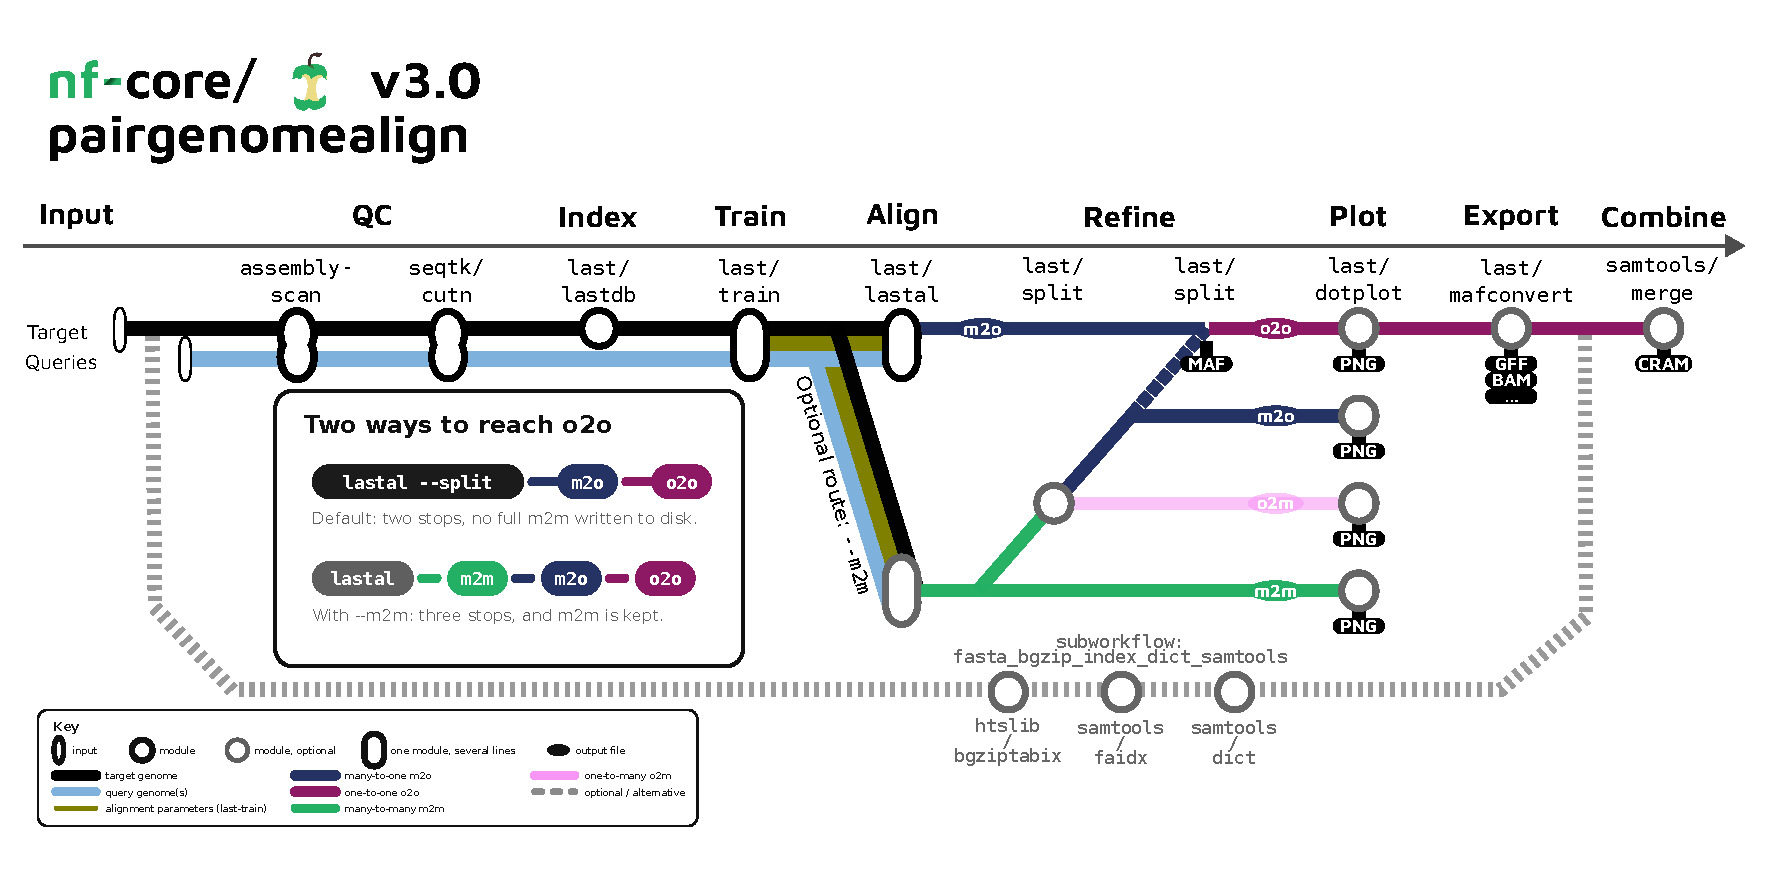
\includegraphics[scale=0.5]{Template_for_both_PCI_and_PCJ/pairgenomealign-tubemap.pdf}
\caption{The nf-core/pairgenomealign pipeline aligns a list of query genomes to a target genomes and produces alignments, plots, and metrics reports. The data flow is indicated by lines and the nf-core modules are indicted by circles.}
\label{fig:fig1}
\end{figure}

We developed the nf-core/pairgenomealign pipeline to align in parallel a list of query genomes to a target genome.  The main steps of the pipeline (Figure~\ref{fig:fig1}), described in detail in the methods section, are 1) index the target genome, 2) compute the optimal training parameters, 3) align the query to the target and 4) reduce the alignment to one-to-one relationship where sequences of each genome are aligned at most once. The pipeline also collects assembly, alignment, and computational resource use statistics.

\subsection*{Use case 1: multiple genome alignment}

\begin{figure}[ht]
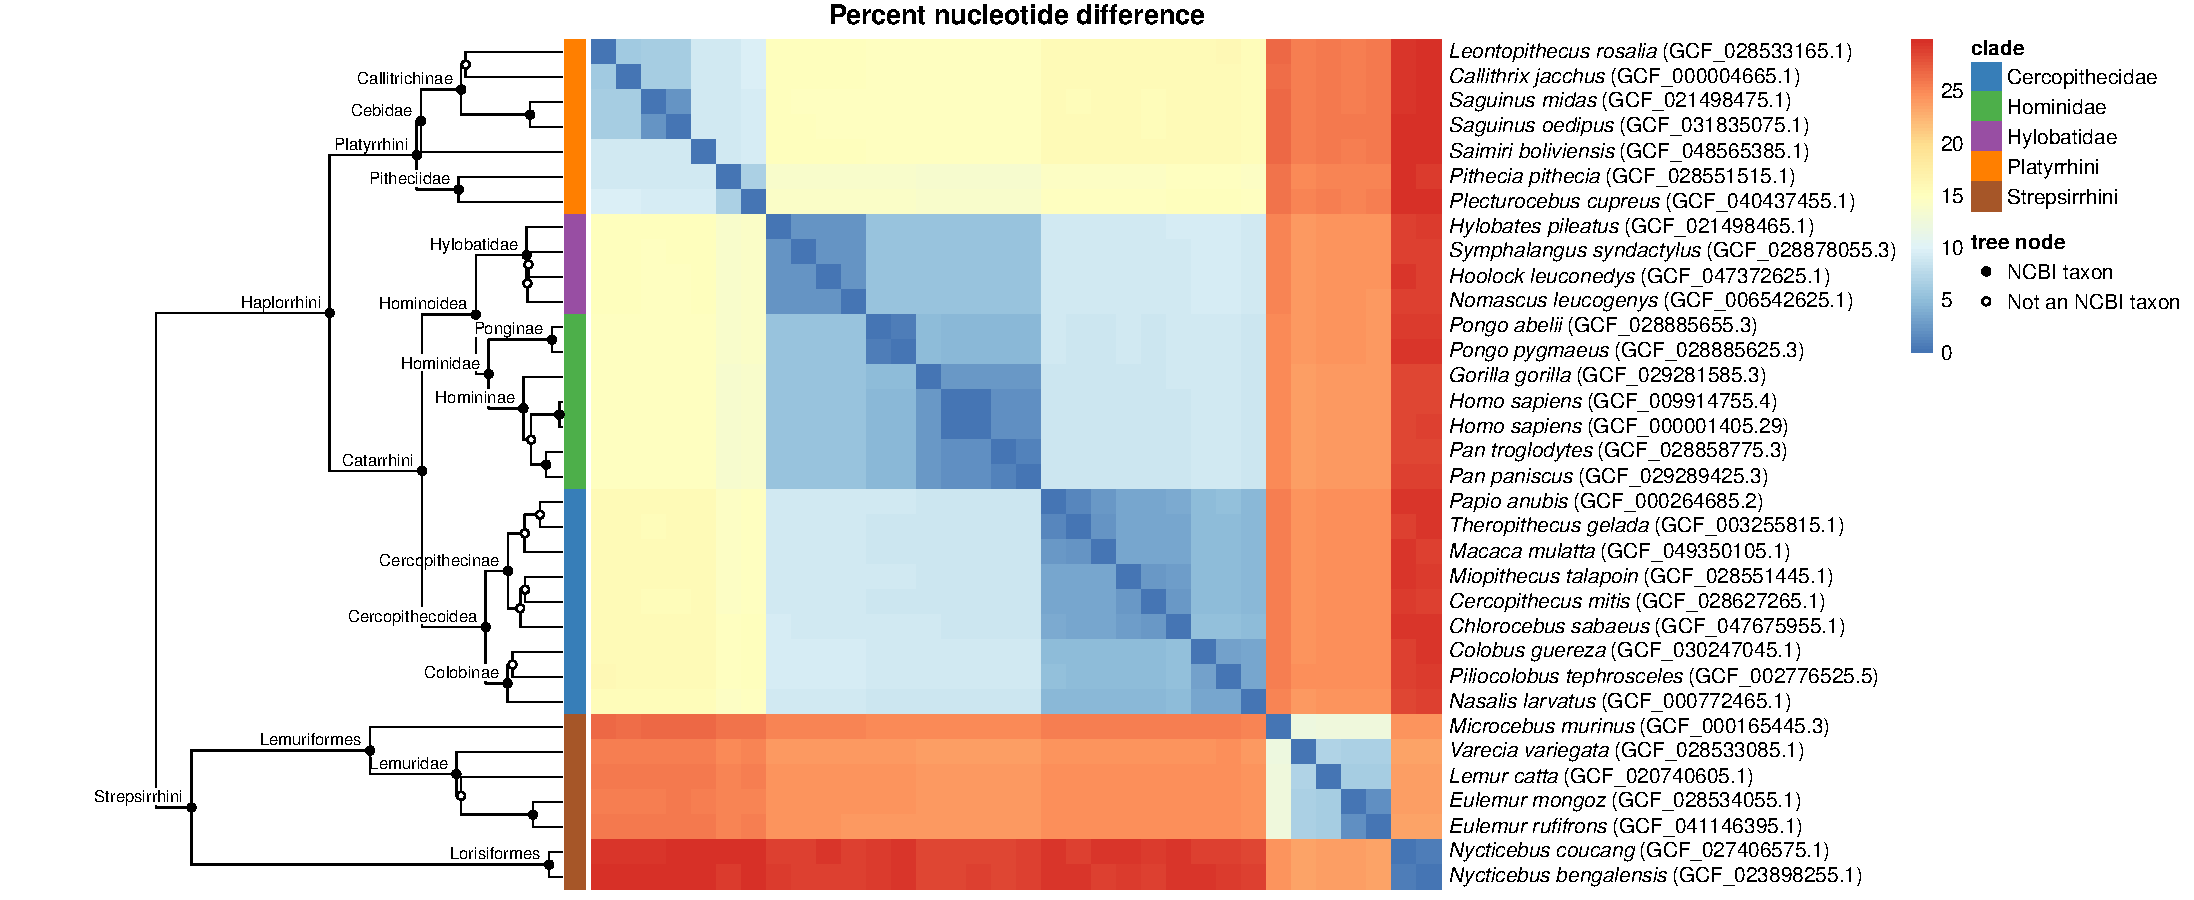
\includegraphics[scale=0.5]{Template_for_both_PCI_and_PCJ/primates_clustering.pdf}
\caption{All-versus-all alignment of primate genomes and outgroups produces a matrix of percent nucleotide identities, which can be clustered to recover an approximation of the taxonomic tree.}
\label{fig:fig2}
\end{figure}

From a list of genomes, all the alignment pairs can be produced by running the pipeline with each one playing the role of the target iteratively.  We illustrate this by aligning 34 primate chromsome-level assmemblies selected to maximally span the primate phylogenetic tree. The human versus other primates iteration, which correspond to the \emph{"full"} test suite of the pipeline, took xyz and xyz time to run on the Amazon computing clound and OISTs HPC cluster respectively. In clades where the molecular clock is stable enough, hierarchical clustering of the percent nucleotide identities recovers phylogenetic trees whose topology ranges from useful to identical to the known taxonomy, as in the case of the primates (Figure~\ref{fig:fig2}).

The pipeline can combine all target-query alignments into, a single CRAM file representing all the alignments in the coordinate system of the target alignments. It is neither a pangenome graph, nor a multiple sequence alignment, but MSAs can be extracted trivially and efficiently, for instance using the \verb|pysam| interface to the HTSlib (\cite{Heger_2009}. It is also useful for inspection of phylogenetic footprints in genome browsers (Figure~\ref{fig:fig3}).

\begin{figure}[ht]
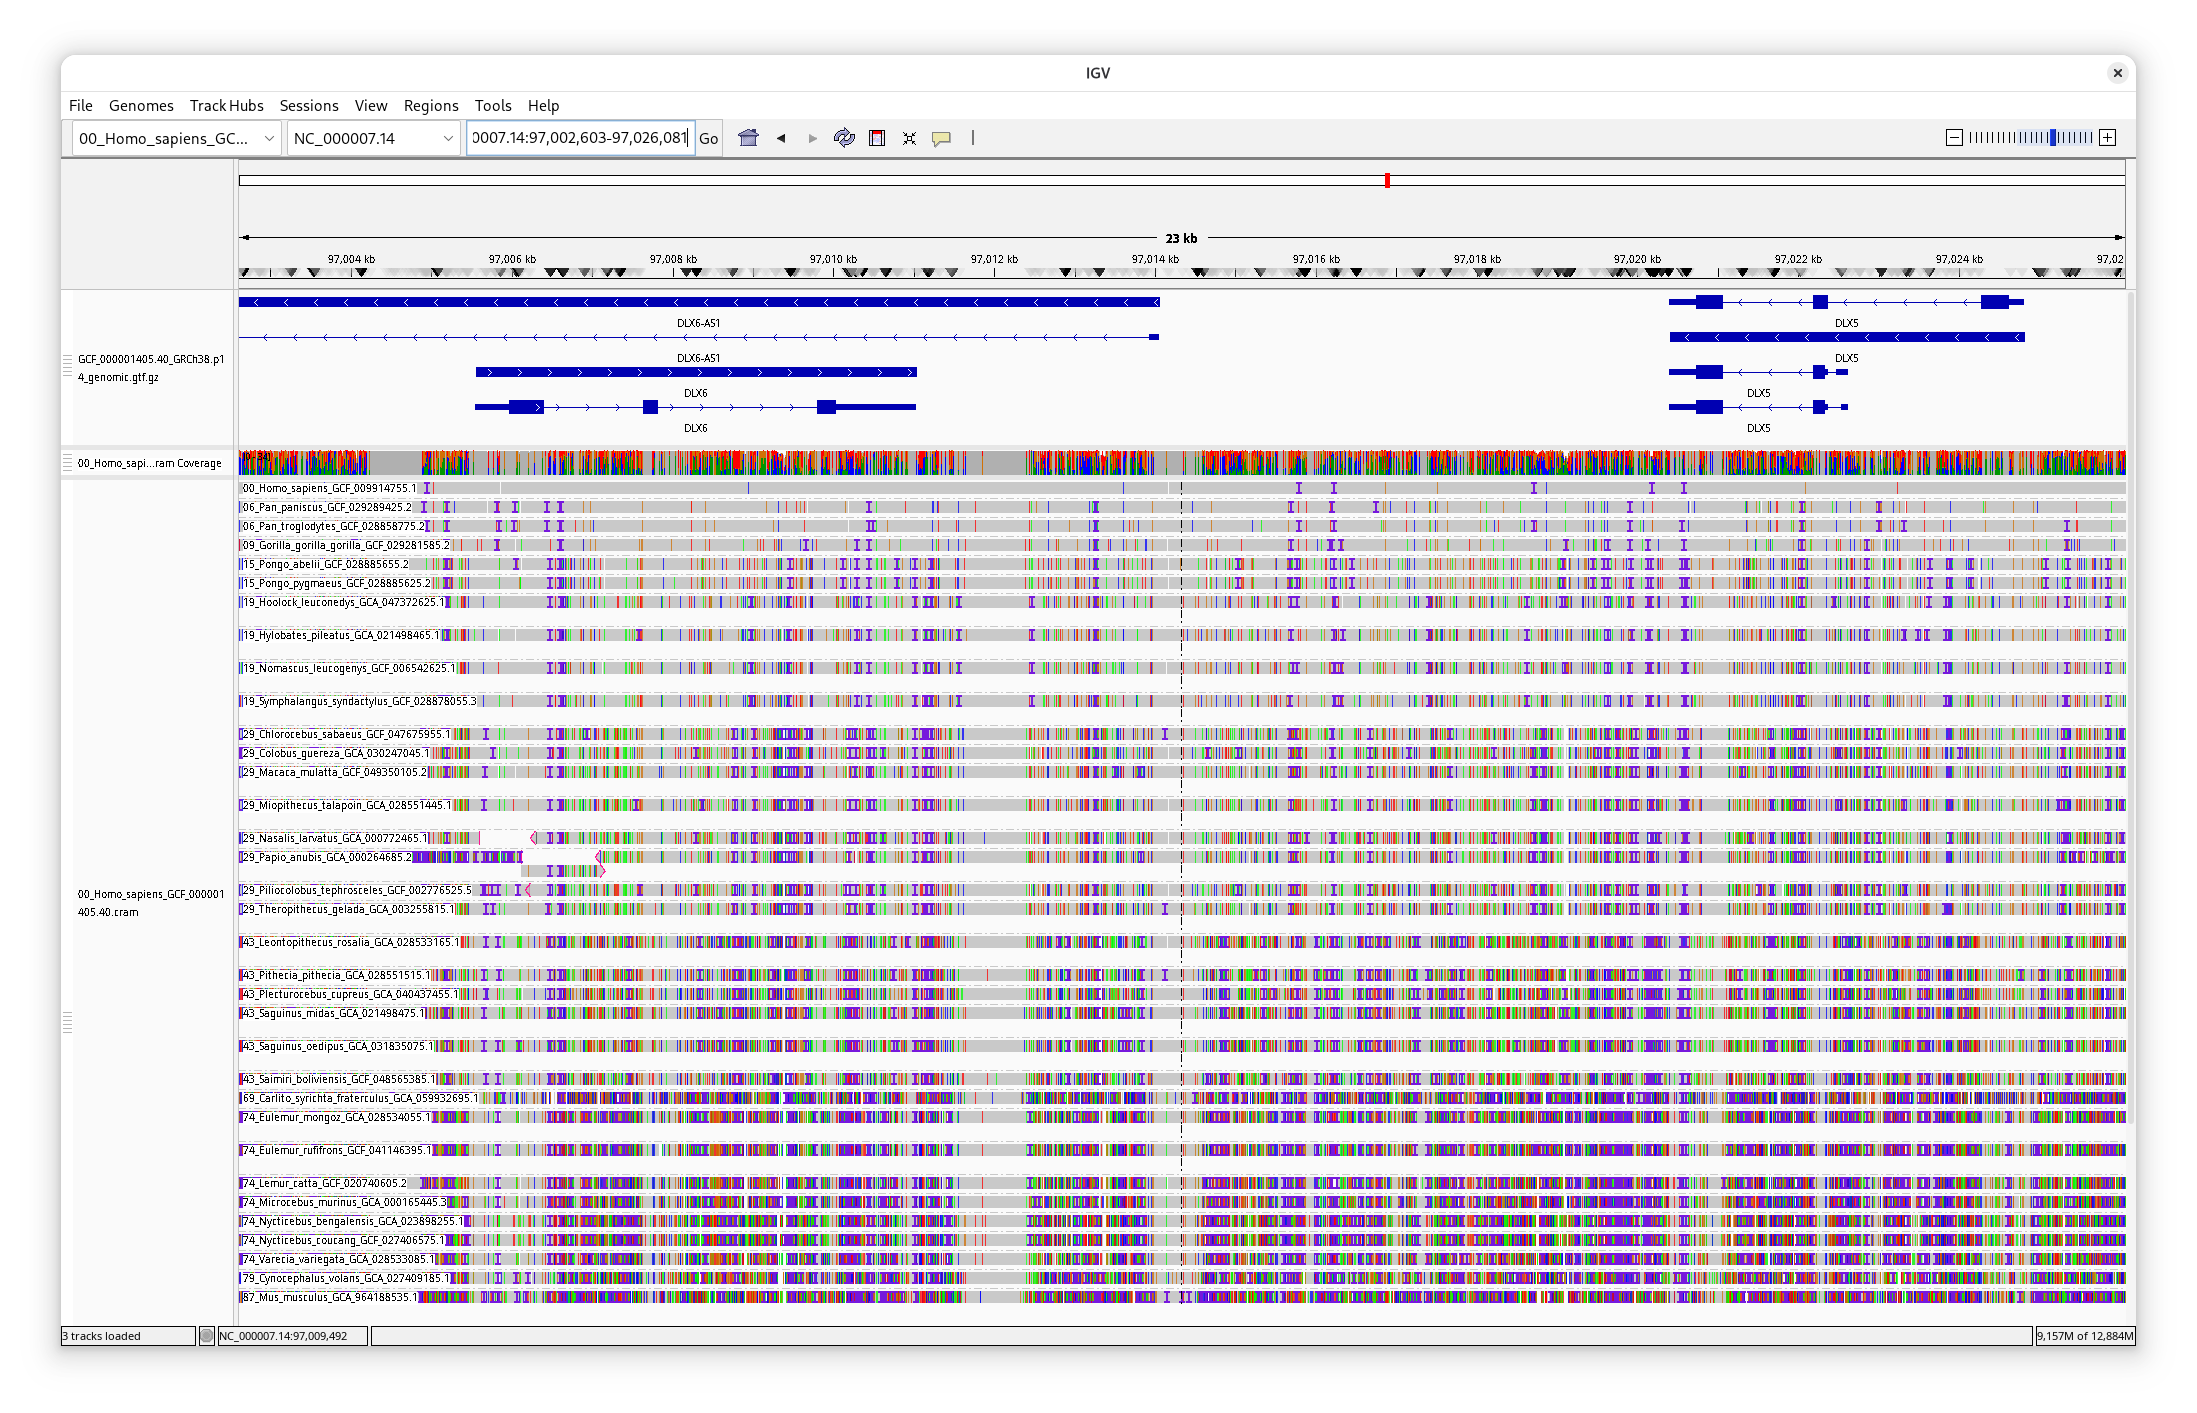
\includegraphics[scale=0.2]{Template_for_both_PCI_and_PCJ/Dlx_screenshot.png}
\caption{Human-versus-all alignment of primate genomes and outgroups compressed in CRAM format displayed in the Integrative Genome Browser. The region displayed is highlights in gray the ultraconserved elements between the DLX5/6 gene pair, through the absence of alignment mismatches or indels (color). The CRAM file used to generate this figure contains the totality of the whole-genome alignments and has a size of 4~GiB.}
\label{fig:fig3}
\end{figure}

\subsection*{Performance benchmarks}

\begin{figure}[ht]
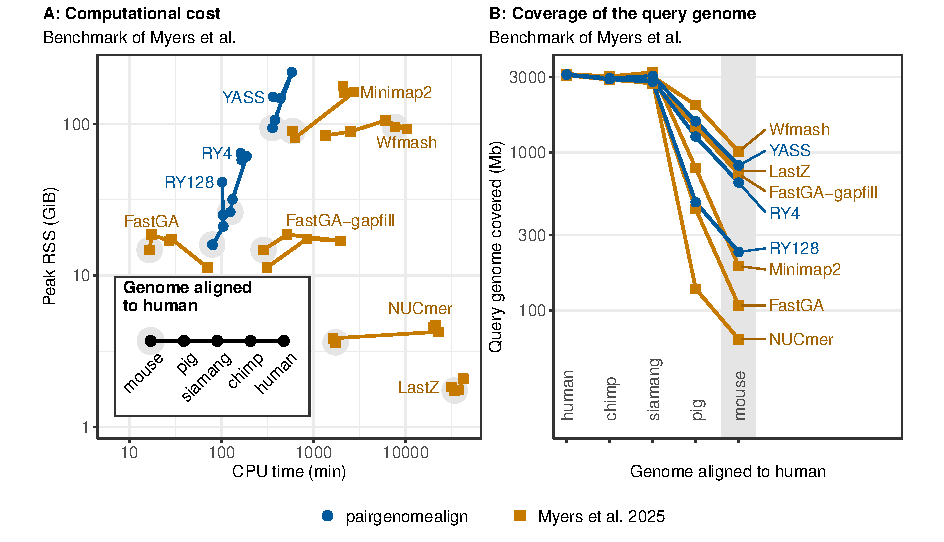
\includegraphics[scale=0.35]{Template_for_both_PCI_and_PCJ/benchmark.pdf}
\caption{Performance statistics of the pairgenomealign pipeline (blue) in context of the \cite{Myers_2025} benchmark. Left panel: peak memory usage and total CPU usgae on a logarithmic scale.  Pairs of genomes aligned with the same software and parameters are linked by dots as in the example inset, with a thicker size for the human–human comparison to indicate the direction. Right panel, alignment coverage (logarithmic scale).}
\label{fig:fig4}
\end{figure}

Human-primate alignments took an average of XYZ minutes, with most of the time, computing and memory resources being used on the alignment step.  Alignment of closer genomes require more resources than aligment of more distant genomes.

Impact of CPU differences.  (accordingly, cpu difference made most difference in the alignment step)

To situate the performance of the pipeline in comparison with other alignment software, we used the benchmark of \cite{Myers_2025} where 5 mammalian genomes are aligned to a human genome reference. We ran our pipeline on the same data using three different indexing seeds, RY128, RY4 and NEAR, and measured 1) the total CPU time of the indexing, training and aligning steps, 2) the maximal memory use during these steps and 3) the total coverage of the many-to-one alignment on the query genomes (Figure~\ref{fig:fig4}). In terms of memory usage, NUCmer and LastZ could align the genomes with the memory available on most computers, FastGA requires quantities found on high-end personal computer (as of 2026), and LAST, Minimap2 and Wfmash need workstation, cloud or high-performance environment. In terms of speed, FastGA was faster than all tools, followed by LAST. The alignment coverage of LAST reached levels comparable to LASTZ when using the RY4 and NEAR seeds. Altogether, our pipeline allows users to tune the speed and sensitivity of the alignments of large genomes according to their needs, outperforming most other tools except FastGA, but requires HPC or cloud platforms for pairs of large genomes.


(explain that each query sequence is often split in many small regions because of x-drop and non-collinearity).



nucleotide identity in methods

put aka ANI somewhere.

Runtime differences between architectures were generally modest for the dominant alignment stage. Intel Cascade Lake consistently outperformed AMD EPYC, with wall-clock times typically 20-30% lower for LASTAL and SPLIT.

No limit on the list of query genomes as Nextflow will chunk batches.

Dot-plot representations, last-dotplot, other export formats, the problem of filtering, the solution in LAST, ...


\subsection*{Use case 2: QC of a new assembly}

There are cases where allowing the target genome to align multiple times on the query, while constraining the query sequences to align only once.  For instance contigs produced by an assembly software can be aligned as query to a target genome.

Align a reference assembly to the new contigs in m2o: there should be two matches per reference sequence.

Make a primary assembly.

Align the primary assembly to the contigs and to the reference assembly in m2o.  Homozygous regions appear as bands with no repeat noise.

(pink lines in dotplots)

multi-cram file of other assemblies (various software) aligned to primary.

WGO...

\subsection*{Use case 3: m2m self-alignment}

The only reasonable choice when aligning diploid to diploid?

Also useful in case of WGD (+?)

or geonomes -> m2m -> m2o / o2m -> o2o


(also useful for QC)



TODO give examples of other pipelines.

 - reproducible pipeline that installs the software for you
 - m2o (how about minimap2)
 - CRAM output: how about other pipelines.
 - parallelisation when many read files need to be mapped to one reference.

 discussion: make not symmetric.

 Example: Oik reads to mitochondria

(Needs special config file)

Benchmark:

add LASTDB indexing time?
add LASTTRAIN or try HUMSUM?
keep mask or tantan?

Aslo, describe teh allvsall script and its restarting of the pipeline with expensive parameters while leveraging the cache.

keep maf files in result folder with conf file? or just run --m2m?  How to get coverage of a MAF file?

MAF -> GFF -> BED (collapse) -> bedtools shmurtz

Give pipeline DOI somewhere.  Is there a stable DOI?

U¥HUMSUM useful with MAM8 on big genomes because last-train also slow?

\section*{Discussion}

How many joules?

Despite being designed for aligning genomes to genomes, the pipeline is also able to align reads to genomes, thank to its flexible design using LAST.  It accepts queries in FASTQ format, and its training step makes it robust to heterogeneity in input data quality and origin (different sequencing platforms have different error profiles).  The many-to-one output alignment guarantees that each base of a read is aligned at most once to the target genome (each base of the target genome can be aligned many times, but only to one base per query sequence).  While other aligners such as minimap2 may perform faster, and specialised pipelines are already available, it can be convenient for the user to just use nf-core/pairgenomealign when already familiar with it and when aligment of a long list of sequencing runs is needed.  For instance, we aligned XYX runs Nanopore and Pacbio; TODO add MiSeq to a reference Oikopleura (italics) genome containing a mitochondrial chromosome sequence, which allowed us to visualise SNPs to ....

  1396160 contigs in Cercopithecus mitis GCF\_028627265.1

Customisation.

User can replace image (for instance Debian Med). Can change LAST version.  Can compile it with local optimisations.
Can run bare but not recommentded (combination of versions not tested)

cutom containers can be used to pin the aligner version while using new developments of the pipeline.

Can run local executor within a job to let processes share CPU and memory.

Possibility to run m2m on the target genome to annotate it by producing a coverage track.  Also run tantan as LAST runs in internally?  Or extract masking info from lastdb.  Or both.   Add other maskiers like ultra and windowmasker, for control?

Add --reverse, for control?

Genome compression... allow other formats?

The pipeline can be run in scripts for all-versus-all comparisons, or could be used for nearest neighbor plus outgroup comparisons before ancestor reconstitution (cactus, Martin's work).

Alignment is not symmetric (one genome is indexed) so one can compute both sides and average results (like in all-versus-all).  The bottleneck is similar genomes, so for most of the pairs it is cheap to compute both.

Also because not symmetric, we call one the target and the other the query.  The target is indexed.  We do not call it reference to avoid confusion with reference genomes (GenBank).

Value of the collected statistics.  Can be used for phylogeny etc.

If users like the CRAM trick, it can be further expanded, for instance: 1) post-processing to either break gaps or merge collinear alignments into longer gaps.  2) what else?

Desined for structural variant detection, but not running this analysis because too open.  Also do not want to recompute alignments when changing SV detection parameters.  We use GenomicBreaks.

Can the pipeline output used in Syri?

Preprocess genomes to remove unplaced scaffolds.  (Many are junk or alternative haplotypes)

Discuss why not repeat masking.  use tantan or alternatives.  Widnowmasker not faster.  -m option as alternative?

Mention HUMSUM (since v1600) somewhere 

HTTP URLs OK.

Centromere repeat unit 400 bp length needed, not default.

why not pangenome

LAST runs well even if there are millions of contigs.  But beware downstream tools and parallelisation strategies.

\begin{table}[ht]
\caption{This is the title of the table. It also contains the legend i.e. an explanation of what the table reveals about the problem at hand (typeset using \texttt{\textbackslash caption}).}
\begin{tabular}{rcccc}
    \hline &&&&\\[-0.95em]
    $n$&1&2&3&4\\ \hline &&&&\\[-0.95em]
    $n^2$&1&4&9&16\\ &&&&\\[-0.95em]
    $n^3$&1&4&9&18\\ \hline  &&&&\\[-0.95em]
\end{tabular}
\caption*{This is the note of the table if required. It is below the table to look nice. This can be done by using the command \texttt{\textbackslash caption*}. Compare with the figure caption above (see Figure~\ref{fig:fig1}).}
\label{tab:tab1}
\end{table}


\section*{Conclusion}

TBW

\section*{Acknowledgements}

We thank the DNA Sequencing Section and the Scientific Computing and Data Analysis Section of the Research Support Division at OIST for their support.

%% This is your acknowledgments. Preprint version xxx[change to the correct number] of this article has been peer-reviewed and recommended by Peer Community In XYZ[change to the name of the PCI] (\url{https://doi.org/10.24072/pci.xxx}[replace by the doi of the recommendation]; \cite{fake}[replace by the citation of the recommendation]).

\section*{Fundings}

This work was supported by OIST core funding.

\section*{Conflict of interest disclosure}

The authors declare that they comply with the PCI rule of having no financial conflicts of interest in relation to the content of the article.

\section*{Data, script, code, and supplementary information availability}

% Data are available online (\url{https://doi.org/10.24072/fake1}[Replace by the DOI of the webpage hosting the data]; \cite{CharleMar_independant-trace-su2_2012}[Replace by the citation of the data])\\
Script and codes are available online (\url{https://doi.org/10.24072/fake2}[Replace by the DOI of the webpage hosting the script and code]; \cite{fixme}[Replace by the citation of the script and code])\\
Supplementary information is available online (\url{https://doi.org/10.24072/fake3}[Replace by the DOI of the webpage hosting the Supplementary information]; \cite{fixme}[Replace by the citation of the Supplementary information])\\ \\
The DOI hyperlinks should be active. They should also be present in the reference list and cited in the text.
\\For the reference section below, do not forget to add a doi for each reference (if available). Do not forget to add the reference of the recommendation, the reference of the data, scripts, code and supplementary material to your bib file, if appropriate.

\printbibliography
\end{document}
